\section{Introduction}

What is OAuth?
{\bf OAuth 2.0 was originally developed as a way of sharing access to specific
data between applications}. OAuth is a commonly used authorization framework
that enables websites and web applications to request limited access to a
user's account on another application. Crucially, OAuth allows the user to
grant this access without exposing their login credentials to the requesting
application. This means users can fine-tune which data they want to share
rather than having to hand over full control of their account to a third
party.

The basic OAuth process is widely used to integrate third-party functionality
that requires access to certain data from a user's account. For example, an
application might use OAuth to request access to your email contacts list so
that it can suggest people to connect with. 

{\bf However, the same mechanism is also
used to provide third-party authentication services}, allowing users to log in
with an account that they have with a different website. 


\subsection{Oauth actors}
It works by defining a series of interactions between four distinct parties: 
\begin{itemize}
    \item {\bf Resource Owner}: An entity capable of granting access to
        protected resources (for example a user)
    \item {\bf Resource Server}: The server which has all
        the protected resources.
    \item {\bf Client}:  An application making protected resource
        request on behalf of its resource owner and with its authorization. 
    \item {\bf Authorization Server}: The server issues the access code and
        access tokens to the client after successfully authenticating. 
\end{itemize}

\subsection{OAuth Tokens}
\begin{itemize}
    \item {\bf Access tokens} are the token the client uses to access the
        Resource Server (API). They have very short lifetime i.e they expire
        within some minutes or hours.
    \item {\bf Refresh Tokens} are the tokens that the client uses to get a new
        Access token. Their lifetime is much longer than access tokens i.e
        days, month and years.
\end{itemize}


\subsection{Oauth grant types / flows}
The requesting, granting, and life management of this tokens are often referred
to as a {\bf flow} or {\bf grant type}. The OAuth specification allows for
several ways of obtaining and validating tokens, and not all flows are meant
for all types of clients.

 The OAuth grant type determines the exact sequence of steps that are involved
 in the OAuth process. The grant type also affects how the client application
 communicates with the OAuth service at each stage, including how the access
 token itself is sent. For this reason, grant types are often referred to as
 "OAuth flows".

An OAuth service must be configured to support a particular grant type before a
client application can initiate the corresponding flow. The client application
specifies which grant type it wants to use in the initial authorization request
it sends to the OAuth service.

There are several different grant types, each with varying levels of complexity
and security considerations. We'll focus on the {\bf authorization code} and
{\bf implicit} grant types as these are by far the most common.

Broadly speaking, both of these grant types involve the following stages:
\begin{enumerate}
    \item The client application requests access to a subset of the user's data, specifying which grant type they want to use and what kind of access they want. 
    \item The user is prompted to log in to the OAuth service and explicitly give their consent for the requested access. 
    \item The client application receives a unique access token that proves
        they have permission from the user to access the requested data.
        Exactly how this happens varies significantly depending on the grant
        type. 
    \item The client application uses this access token to make API calls
        fetching the relevant data from the resource server. 
\end{enumerate}

\subsubsection{OAuth scopes}
For any OAuth grant type, the client application has to specify which data it
wants to access and what kind of operations it wants to perform. It does this
using the scope parameter of the authorization request it sends to the OAuth
service.

For basic OAuth, the scopes for which a client application can request access
are unique to each OAuth service. As the name of the scope is just an arbitrary
text string, the format can vary dramatically between providers. Some even use
a full URI as the scope name, similar to a REST API endpoint. For example, when
requesting read access to a user's contact list, the scope name might take any
of the following forms depending on the OAuth service being used:
\begin{verbatim}
scope=contacts
scope=contacts.read
scope=contact-list-r
scope=https://oauth-authorization-server.com/auth/scopes/user/contacts.readonly
\end{verbatim}

When OAuth is used for authentication, however, the standardized {\bf OpenID
Connect scopes} are often used instead. For example, the scope openid profile
will grant the client application read access to a predefined set of basic
information about the user, such as their email address, username, and so on.

\subsubsection{Authorization code grant type}
This flow is the most widely spread OAuth flow.

First of all note that in the following diagram:
\begin{itemize}
        \item the Authorization server is hosted by the ressource server but it
            the majority of the cases they are two diffrent servers.
        \item the initial step of user interacting with the service on the
            client that need to access user's data have been omited.
\end{itemize}

In short:
\begin{itemize}
    \item the client application and OAuth service provider first use redirects
        to exchange a series of browser-based HTTP requests that initiate the
        flow. 
    \item The ressource owner is asked whether they consent to the requested access. 
    \item If they accept, the client application is granted an "authorization code". 
    \item The client application then exchanges this code with the OAuth
        service to receive an "access token"
    \item the access token can use to make API calls to fetch the relevant user data.
\end{itemize}

\begin{figure}
  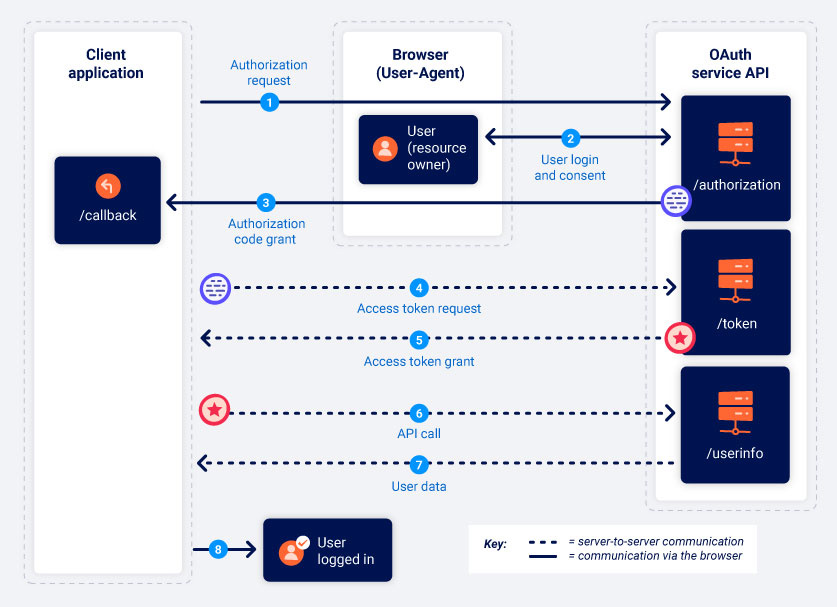
\includegraphics[width=\linewidth]{web_server_side/oauth/images/oauth-authorization-code-flow.jpg}
  \caption{Authorization code grant type}
  \label{fig:oauth-authorization-code-flow}
\end{figure}

{\bf Authorization request}: 
The client application sends a request to the OAuth service's authorization
endpoint asking for permission to access specific user data. Note that the
endpoint mapping may vary between providers.
owever, you should always be able to identify the endpoint based on the parameters used in the request.
\begin{verbatim}
GET /authorization?
    client_id=12345&
    redirect_uri=https://client-app.com/callback&
    response_type=code&
    scope=openid%20profile&
    state=ae13d489bd00e3c24 HTTP/1.1
Host: oauth-authorization-server.com
\end{verbatim}

 This request contains the following noteworthy parameters, usually provided in
 the query string:
 \begin{itemize}
    \item \verb+client_id+: Mandatory parameter containing the unique identifier of
        the client application. This value is generated when the client
        application registers with the OAuth service.
    \item \verb+redirect_uri+:  The URI to which the user's browser should be
        redirected when sending the authorization code to the client
        application. This is also known as the {\bf callback URI} or {\bf
        callback endpoint}. Many OAuth attacks are based on exploiting flaws in
        the validation of this parameter.
    \item \verb+response_type+:  Determines which kind of response the client
        application is expecting and, therefore, which flow it wants to
        initiate. For the authorization code grant type, the value should be
        \verb+code+.
    \item \verb+scope+:  Used to specify which subset of the user's data the
        client application wants to access.
    \item \verb+state+:  Stores a unique, unguessable value that is tied to the
        current session on the client application. The OAuth service should
        return this exact value in the response, along with the authorization
        code. This parameter serves as a form of CSRF token for the client
        application by making sure that the request to its /callback endpoint
        is from the same person who initiated the OAuth flow.
\end{itemize}


{\bf User login and consent}:
 When the authorization server receives the initial request, it will redirect
 the user to a login page, where they will be prompted to log in to their
 account with the OAuth provider.  They will then be presented with a list of
 data that the client application wants to access. This is based on the scopes
 defined in the authorization request. 

It is important to note that once the user has approved a given scope for a
client application, this step will be completed automatically as long as the
user still has a valid session with the OAuth service. In other words, the
first time the user selects "Log in with social media", they will need to
manually log in and give their consent, but if they revisit the client
application later, they will often be able to log back in with a single click.

{\bf Authorization code grant}:
If the user consents to the requested access, their browser will be redirected
to the callback endpoint that was specified in the \verb+redirect_uri+
parameter of the authorization request. The resulting \verb+GET+ request will
contain the authorization code as a query parameter. Depending on the
configuration, it may also send the state parameter with the same value as in
the authorization request.
\begin{verbatim}
GET /callback?code=a1b2c3d4e5f6g7h8&state=ae13d489bd00e3c24 HTTP/1.1
Host: client-app.com
\end{verbatim}

{\bf Access token request}:
 Once the client application receives the authorization code, it needs to
 exchange it for an access token. To do this, it sends a server-to-server
 \verb+POST+ request to the OAuth service's token endpoint. All communication
 from this point on takes place in a secure back-channel and, therefore, cannot
 usually be observed or controlled by an attacker.
\begin{verbatim}
POST /token HTTP/1.1
Host: oauth-authorization-server.com
…
client_id=12345&client_secret=SECRET&redirect_uri=https://client-app.com/callback&grant_type=authorization_code&code=a1b2c3d4e5f6g7h8
\end{verbatim}

In addition to the \verb+client_id+ and \verb+authorization_code+, you will notice the following new parameters:
\begin{itemize}
    \item \verb+client_secret+:  The client application must authenticate
            itself by including the secret key that it was assigned when
            registering with the OAuth service.
    \item \verb+grant_type+:  Used to make sure the new endpoint knows which
        grant type the client application wants to use. In this case, this
        should be set to \verb+authorization_code+.
    \item \verb+redirect_uri+: This must be identical to the redirect URI
        provided in the original link.
\end{itemize}


{\bf Access token grant}

The OAuth service will validate the access token request. If everything is as expected, the server responds by granting the client application an access token with the requested scope.
\begin{verbatim}
{
    "access_token": "z0y9x8w7v6u5",
    "token_type": "Bearer",
    "expires_in": 3600,
    "scope": "openid profile",
    …
}
\end{verbatim}

{\bf API call}:
 Now the client application has the access code, it can finally fetch the
 user's data from the resource server. To do this, it makes an API call to the
 OAuth service's userinfo endpoint. The access token is submitted in the
 \verb+Authorization: Bearer+ header to prove that the client application has
 permission to access this data.
\begin{verbatim}
GET /userinfo HTTP/1.1
Host: oauth-resource-server.com
Authorization: Bearer z0y9x8w7v6u5
\end{verbatim}

{\bf Resource grant}:
The resource server should verify that the token is valid and that it belongs
to the current client application. If so, it will respond by sending the
requested resource i.e. the user's data based on the scope of the access
token.
\begin{verbatim}
{
    "username":"carlos",
    "email":"carlos@carlos-montoya.net",
    …
}
\end{verbatim}

The client application can finally use this data for its intended purpose. {\bf
    In the case of OAuth authentication, it will typically be used as an ID to
grant the user an authenticated session, effectively logging them in}.


\subsubsection{Implicit grant type}
 The implicit grant type is much simpler. Rather than first obtaining an
 authorization code and then exchanging it for an access token, the client
 application receives the access token immediately after the user gives their
 consent.

You may be wondering why client applications don't always use the implicit
grant type. The answer is relatively simple - it is far less secure. When using
the implicit grant type, all communication happens via browser redirects -
there is no secure back-channel like in the authorization code flow. This means
that the sensitive access token and the user's data are more exposed to
potential attacks.

The implicit grant type is more suited to single-page applications and native
desktop applications, which cannot easily store the \verb+client_secret+ on the
back-end, and therefore, don't benefit as much from using the authorization
code grant type.

\begin{figure}
  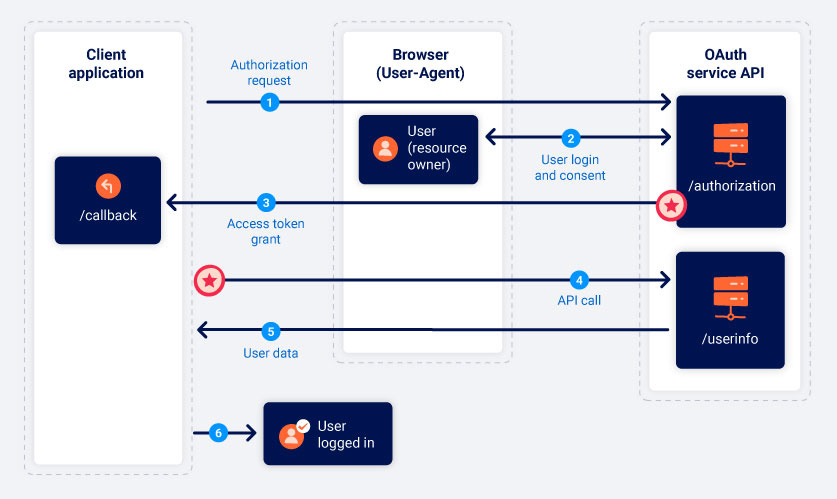
\includegraphics[width=\linewidth]{web_server_side/oauth/images/oauth-implicit-flow.jpg}
  \caption{Implicit grant type}
  \label{fig:oauth-implicit-flow.jpg}
\end{figure}


{\bf Authorization request}: 
Same as before but \verb+response_type+ is set to \verb+token+


{\bf User login and consent}:
This process is exactly the same as for the authorization code flow.


{\bf Access token grant}:
If the user gives their consent to the requested access, this is where things
start to differ. The OAuth service will redirect the user's browser to the
\verb+redirect_uri+ specified in the authorization request. However, instead of
sending a query parameter containing an {\bf authorization code}, it will send
the {\bf access token} and other token-specific data as a URL fragment.
\begin{verbatim}
GET /callback#
    access_token=z0y9x8w7v6u5&
    token_type=Bearer&
    expires_in=5000&
    scope=openid%20profile&
    state=ae13d489bd00e3c24 HTTP/1.1
Host: client-app.com
\end{verbatim}

As the access token is sent in a URL fragment, it is never sent directly to the
client application. Instead, the client application must use a suitable script
to extract the fragment and store it. 

{\bf API call}:
 Once the client application has successfully extracted the access token from the URL fragment, it can use it to make API calls to the OAuth service's userinfo endpoint. Unlike in the authorization code flow, this also happens via the browser.
\begin{verbatim}
GET /userinfo HTTP/1.1
Host: oauth-resource-server.com
Authorization: Bearer z0y9x8w7v6u5
\end{verbatim}


{\bf Resource grant}:
 The resource server should verify that the token is valid and that it belongs
 to the current client application. If so, it will respond by sending the
 requested resource i.e. the user's data based on the scope associated with the
 access token.
\begin{verbatim}
{
    "username":"carlos",
    "email":"carlos@carlos-montoya.net"
}
\end{verbatim}

The client application can finally use this data for its intended purpose. In
the case of OAuth authentication, it will typically be used as an ID to grant
the user an authenticated session, effectively logging them in. 



\subsubsection{Resource Owner Credentials Grant Type}
The Resource Owner Credentials Grant type is suitable in cases where the
resource owner has a trust relationship with the client. Care should be taken
when enabling this grant type. It should only be used when other flows are not
viable. In this type, the user needs to share their credentials directly with
the client, which the client then submits to the authorization server in
exchange for an access token.

\begin{figure}
  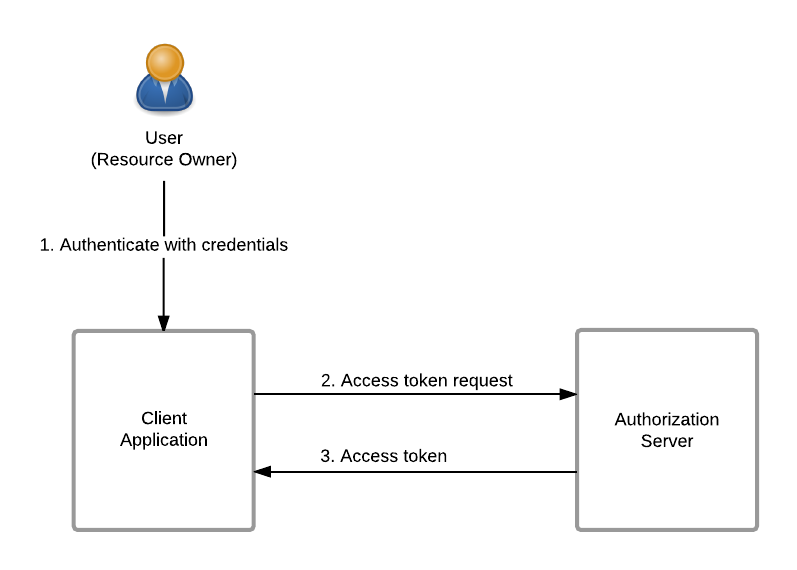
\includegraphics[width=\linewidth]{web_server_side/oauth/images/oauth-resource-owner-credentials-flow.png}
  \caption{Resource Owner Credentials Grant Type}
  \label{fig:oauth-resource-owner-credentials-flow}
\end{figure}

This grant type is used to migrate existing clients using direct authentication
schemes such as HTTP Basic or Digest authentication to OAuth by converting the
stored credentials to an access token. 

\subsubsection{Client Credentials Grant Type}

With the Client Credentials Grant type, a client application will authenticate
to the authorization server and request an access token. This grant type is
used in machine-to-machine authentication, where a specific user’s permissions
to access the data is not required. The flow of Client Credentials Grant is
shown below.

\subsubsection{Refresh Token Grant Type}
Clients use the Refresh Token Grant type to retrieve an access token. This
allows clients to obtain a new access token without further interaction with
the user. The flow of the Refresh Token Grant is as below.


\begin{enumerate}
    \item The client application will use other grant types (authorization code
        grant or implicit code grant) to obtain the refresh token.

        \item Client application sends a request to the authorization server to
            exchange the refresh token with an access token providing :
            \begin{itemize}
                \item \verb+grant_type+:The grant type for this flow is
                    \verb+refresh_token+
                \item \verb+refresh_token+: Refresh token obtained from the
                    authorization server using another grant type.
                \item \verb+client_id+: The client ID which is received from
                    the authorization server when the application is first
                    created.
                \item \verb+client_secret+: Since this request is made from
                    server-side code, the secret is included
            \end{itemize}
\end{enumerate}

\subsection{OAuth authentication}
